\chapter{Open defects}
\label{ch:defects}

\section{Burst mode replays about half of every run}
\label{sec:replay}

\subsection{The evidence}

Every burst run in both sessions shows the same signature: acquires strictly
alternate short and long, and the short ones return a \emph{bit-identical} copy of
the previous batch.

\begin{center}
\small
\begin{tabular}{@{}lrrrrrr@{}}
\toprule
\hd{Run} & \hd{Batches} & \hd{Stale} & \hd{Fraction} & \hd{Pattern} & \hd{Recorded} & \hd{True} \\
\midrule
2026-08-06 \co{_142358} & 211 & 106 & 50.2\% & 13 / 425\,ms & 3911\,Hz & \textbf{1946\,Hz} \\
2026-08-06 \co{_142443} & 66  & 33  & 50.0\% & 13 / 424\,ms & 4182\,Hz & \textbf{2091\,Hz} \\
2026-08-06 \co{_145051} & 44  & 23  & 52.3\% & 13 / 425\,ms & 4421\,Hz & \textbf{2110\,Hz} \\
2026-08-06 \co{_145144} & 14  & 7   & 50.0\% & 13 / 425\,ms & 4455\,Hz & \textbf{2227\,Hz} \\
\textbf{2026-08-14 \co{_150458}} & \textbf{371} & \textbf{185} & \textbf{49.9\%} & 12 / 120\,ms & 6161\,Hz & \textbf{3089\,Hz} \\
\bottomrule
\end{tabular}
\end{center}

The separation is clean with nothing in between: the duplicate fraction is
\textbf{0.957 in the fast batches} and 0.069 in the real ones. Within a stale batch
the only rows that differ from the previous batch are row 0 and a block around rows
770--818 --- and 819 is exactly the streamer's transfer stride,
$0.1\times\co{avg_maxlen}/\co{reads_per_shot}$.

Detection uses two independent tests, either of which condemns a batch:
\begin{enumerate}
  \item $\ge$90\% of rows identical to the previous batch;
  \item wall-clock duration under half the FPGA work the batch claims to contain.
\end{enumerate}
Both are needed. On \co{_145051}, batch 24 is 82\% duplicate --- under the fraction
threshold, because the run's one CSV-flush stall shifted the alignment --- but
returned in \SI{12.9}{\milli\second} against \SI{425}{\milli\second} of claimed
pulse work.

\subsection{The 2026-08-06 root cause, and why it is now disproved}

\begin{retractbox}[DISPROVED --- \co{config_all} / \co{reset_tproc} was not the mechanism]
The 2026-08-06 analysis found a real bug. \co{qickdawg} called
\co{config_all(..., load_pulses=...)}, but \co{qick} 0.2.386 names that parameter
\co{load_envelopes}. \textbf{Every acquire raised \co{TypeError}}, was silently
caught, and fell back to \co{config_all(soc)} with \co{reset=False} --- and
\co{reset=False} means \co{stop_tproc(lazy=True)}, which \co{qick} documents as a
no-op on tProc v1. \textbf{The tProc was never stopped between runs}, so the
accumulated buffer was re-armed under a possibly-still-running program.

That was fixed on 2026-08-12 (commit \co{942d9e8}) and a \co{reset_tproc=}
argument was threaded through \co{acquire()}.

\textbf{The 2026-08-14 run used the fix and the replay fraction did not change}:
49.9\% (185/371). The rig was definitely running the new code --- $\tau$ =
\SI{120}{\micro\second} took effect and the new streaming cell produced output.

So the keyword bug was real and worth fixing, but it was \emph{not} the cause of
the replay. \textbf{The root cause is unknown.}
\end{retractbox}

What the elimination does tell us: the mechanism is not the tProc failing to stop,
because forcing the stop changes nothing. The remaining candidates involve the
accumulated buffer or the shot counter rather than the program:

\begin{itemize}
  \item \co{config_bufs()} re-arming the accumulator without clearing the counter,
        so \co{poll_data} returns the previous run's completed shots as if they were
        new;
  \item the board-side worker thread from the previous \co{start_readout} not being
        joined, so its queue still holds the old transfer;
  \item \co{start_readout}'s shot counter being read before the tProc has reset it.
\end{itemize}
None has been tested. A single instrumented burst run on the rig, printing the shot
counter and the queue depth before and after each \co{start_readout}, would
discriminate.

\subsection{Mitigation, which is in place}

\co{cfg.multipoint_on_stale = "drop"} makes the freshness guard re-acquire
(\co{multipoint_stale_retries}, default 2) and, if every attempt still returns the
same buffer, return \co{None} so the caller \textbf{skips the batch}. A replay is
never written to the CSV as though it were data.

This costs duty cycle, not correctness --- the recorded rate becomes honest:
3089\,Hz rather than the 6161\,Hz the raw file claims. Simulated against a board
that replays every second call, all 20 requested batches were recovered as real
data.

The guard is a byte comparison (\co{blake2b}) against the previous raw buffer, so it
costs microseconds and catches the failure \emph{whatever} its mechanism --- which
is why it survived the root cause being wrong.

\section{Streaming's noise floor is about 6\texorpdfstring{$\times$}{x} the burst floor}
\label{sec:streamnoise}

\subsection{The evidence}

Streaming and burst ran ten minutes apart at the same $\tau$, on the same hardware,
with nothing changed on the bench (confirmed with the operator). Their amplitude
spectral densities differ by a \textbf{flat factor of $\sim$6 across the whole
band} (\file{tables/read_path.csv}):

\begin{center}
\small
\begin{tabular}{@{}lrrr@{}}
\toprule
\hd{Band} & \hd{Stream} & \hd{Burst (cleaned)} & \hd{Ratio} \\
\midrule
10--30\,Hz   & 234.8 & 38.6 & 6.08 \\
30--60\,Hz   & 234.1 & 44.1 & 5.31 \\
60--100\,Hz  & 240.8 & 39.8 & 6.06 \\
100--200\,Hz & 231.1 & 38.7 & 5.97 \\
200--350\,Hz & 242.4 & 38.8 & 6.25 \\
350--500\,Hz & 250.2 & 39.7 & 6.30 \\
\bottomrule
\end{tabular}
\end{center}
\emph{(\etaunit.)}

\begin{figure}[H]
\centering

\includegraphics[width=\linewidth]{figures/read_path_asd.png}
\caption{Streaming against burst amplitude spectral density. Both floors are flat;
the ratio is constant across two and a half decades.}
\end{figure}

\subsection{2026-08-17: still there, but far smaller}
\label{sec:streamnoise0817}

The 2026-08-17 morning session gives an independent look at the same comparison,
after the photodiode gain change and on a different computer. It is a weaker
measurement than the 08-14 one --- the runs are ten minutes apart rather than
interleaved, and the whole session was a magnet test with the magnet moved by
hand --- so each run is quoted twice: over the full \SI{30}{\second}, and over
the first \SI{5}{\second} before the magnet was brought in at all. From
\file{tables/0817\_read\_paths.csv}, medians over 4 stream and 6 de-staled burst
runs:

\begin{center}
\small
\begin{tabular}{@{}lrrrcrrr@{}}
\toprule
& \multicolumn{3}{c}{\hd{full \SI{30}{\second}}} & & \multicolumn{3}{c}{\hd{first \SI{5}{\second}, magnet away}} \\
\cmidrule{2-4}\cmidrule{6-8}
\hd{Band} & \hd{Stream} & \hd{Burst} & \hd{Ratio} & & \hd{Stream} & \hd{Burst} & \hd{Ratio} \\
\midrule
10--30\,Hz   & 113.3 & 78.4 & 1.45 & & 127.6 & 95.9 & 1.33 \\
100--200\,Hz & 105.5 & 77.2 & 1.37 & & 131.2 & 86.2 & 1.52 \\
350--500\,Hz & 105.6 & 78.0 & 1.35 & & 137.3 & 87.8 & 1.56 \\
\bottomrule
\end{tabular}
\end{center}
\emph{(\etaunit.)}

\begin{figure}[H]
\centering
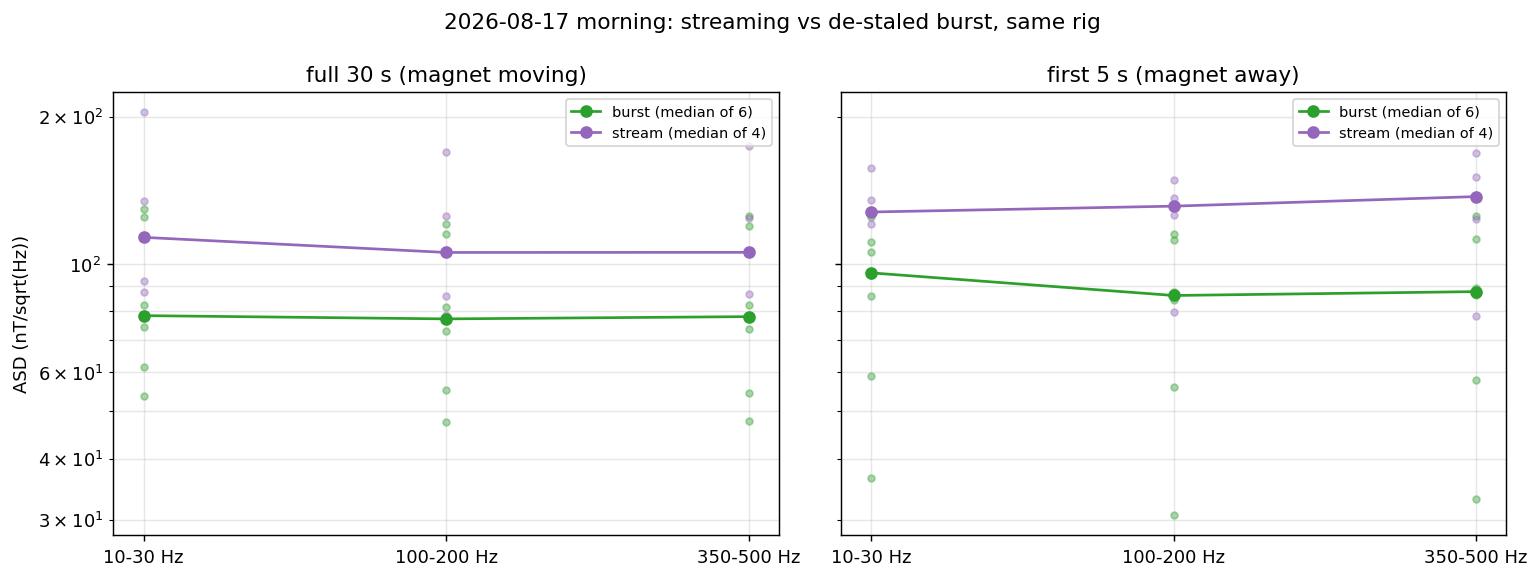
\includegraphics[width=\linewidth]{figures/0817_read_paths.png}
\caption{2026-08-17 morning. Points are individual runs, lines the median. The
run-to-run scatter within each mode is a factor of $\sim$2, which is the main
reason this session cannot replace the interleaved A/B.}
\end{figure}

\begin{keybox}[The excess is real but it is 1.3--1.6\texorpdfstring{$\times$}{x}, not 6\texorpdfstring{$\times$}{x}]
Streaming is still worse than burst, still by a flat factor across the band ---
the signature has not changed. But the size has: \textbf{1.3--1.6$\times$} here
against \textbf{5.3--6.3$\times$} on 08-14. Both windows agree, so it is not the
magnet.

Three things differ between the sessions and none has been isolated: the
photodiode gain change, \co{mw_gain} (this session ran at \num{10500}; the
current notebook default is \num{15000}), and the \co{stream()} configuration
sequence, which was aligned with \co{acquire()}'s on 2026-08-16 --- \emph{after}
the 08-14 data and \emph{before} this session. That last one is the leading
candidate precisely because it was the only difference in the read path, and
this is the first data taken with it.

Do not treat the 6$\times$ figure as current. Do not treat 1.4$\times$ as settled
either: \co{profile\_twopoint\_acquire.py --compare-read-paths} interleaves the
two modes on the same program and is still the measurement that closes this.
\end{keybox}

\subsection{What has been ruled out, with the measurement}

\begin{center}
\small
\begin{tabular}{@{}p{4.0cm}p{7.4cm}l@{}}
\toprule
\hd{Candidate} & \hd{Measurement} & \hd{Verdict} \\
\midrule
Mains pickup & The 60\,Hz comb (8 harmonics) accounts for \textbf{4.5\%} of the
  stream's $\Delta f$ variance & ruled out \\
Slow drift / the PL droop & Below $\sim$10\,Hz is \textbf{2.8\%} of the $\Delta f$
  variance (it is 85\% of the \emph{common-mode} variance, but that cancels) & ruled out \\
Dropped reps & \textbf{0} \co{rep_index} gaps in 125\,000 reps & ruled out \\
Duplicated samples & \textbf{0} duplicate rows in 31\,250 samples & ruled out \\
Packet-boundary artefacts & $\sigma$ at the first 5 rows of a packet is
  \textbf{0.96$\times$} the mid-packet $\sigma$ (30.7 vs 31.8 ADC) & ruled out \\
Buffer overflow as packets fill & The 500-sample first packet is \emph{no noisier}
  than the 205-sample ones & ruled out \\
Torn reads (partial accumulations) & The residual is symmetric, skew \textbf{+0.12},
  kurtosis 1.24. Torn reads would skew strongly low & ruled out \\
\bottomrule
\end{tabular}
\end{center}

A flat, structureless, frequency-independent multiplicative excess is what a
\textbf{read-path} difference looks like, not what a physical disturbance looks
like. Both paths pull from the same accumulated buffer; they differ in how they
configure and drain it.

\subsection{What has been done about it}

\co{stream()}'s configuration sequence now mirrors
\co{NVAveragerProgram.acquire()} step for step. It did not before:

\begin{center}
\small
\begin{tabular}{@{}lll@{}}
\toprule
& \hd{\co{acquire()}} & \hd{\co{stream()}, before 2026-08-16} \\
\midrule
\co{config_all}   & yes & yes \\
\co{start_src}    & yes & yes \\
\co{config_bufs}  & yes & yes, \emph{different order} \\
\co{reload_mem}   & \textbf{yes} & \textbf{missing entirely} \\
\co{start_readout}& yes & yes \\
\bottomrule
\end{tabular}
\end{center}

That is the cheapest candidate to eliminate and it costs nothing if irrelevant.
\co{stream()} also now refuses to reshape a packet whose payload size does not
match its own rep count, which would misalign every subsequent sample and mix the
two parked frequencies --- a failure that would produce exactly this signature and
that was previously invisible.

\begin{openbox}[OPEN --- neither change is verified to fix it]
\textbf{Highest-priority open item.} The test is designed and takes about a minute:
\begin{center}
\co{python scripts/profile_twopoint_acquire.py --compare-read-paths --tau 120 --reps 500}
\end{center}
It alternates \co{acquire(per_rep=True)} and \co{stream()} on the \emph{same
program object}, five times, within seconds. Identical FPGA work; only the read path
differs. It compares raw normalised counts rather than kHz, so it does not depend on
the ODMR calibration still being valid.

\begin{itemize}
  \item ratio $\approx 1.0$ $\Rightarrow$ the $\sim$6$\times$ was the environment
        after all, and streaming needs no caveat;
  \item ratio $\gg 1$ $\Rightarrow$ streaming really is noisier on identical work,
        and it is a software defect. Follow with \co{--stream-scan} to see whether
        it grows with buffer fill.
\end{itemize}
\end{openbox}

\section{An interrupted cell wedges the board, and a kernel restart does not clear it}
\label{sec:wedge}

Found 2026-08-17, when Step~4C hung at its auto-zero \co{acquire()} and \co{Ctrl-C}
produced a traceback ending in \co{sock.recv(size, socket.MSG\_WAITALL)}. Fixed the
same day. It is recorded here because it silently contaminates data rather than
only costing time, and because the recovery is not obvious.

\subsection{The mechanism}

\co{qick}'s \co{poll\_data()} takes a \co{timeout} argument that defaults to
\co{None}, and its board-side body is

\begin{center}
\co{length, data = streamer.data\_queue.get(block=True, timeout=timeout)}
\end{center}

\noindent so with the default it blocks \emph{forever}. \co{qickdawg}'s drain loop
called \co{qd.soc.poll\_data()} with no arguments, so every acquire inherited that
default. The queue is fed by the board's readout worker, which only transfers once
the tProc shot counter advances past a stride. If the counter never advances --- a
program that did not start, a tProc left running by an earlier cell, an abandoned
\co{stream()} generator --- nothing is ever queued and the RPC never replies.

The client then sits in \co{sock.recv(..., MSG\_WAITALL)} waiting for a reply that
is not coming. That is the traceback above, and the four consequences are:

\begin{enumerate}
  \item \textbf{The wait is unbounded.} No timeout, anywhere in the path.
  \item \textbf{\co{Ctrl-C} only unblocks the client.} The board-side Pyro worker
        thread stays blocked in \co{queue.get()} for the life of the daemon.
  \item \textbf{That thread is still a consumer.} When the next run finally queues a
        packet, the abandoned \co{get()} can take it instead of the live caller ---
        so a subsequent run silently loses its first packet.
  \item \textbf{Restarting the notebook kernel does not help}, because the wedged
        thread is on the board, not in the client.
\end{enumerate}

\subsection{Reproduced offline}

Against the real \co{qick.streamer.DataStreamer} driven by a fake board whose shot
counter never advances (\file{scripts/} is not needed; the check is eight lines):

\begin{center}
\begin{tabular}{@{}lll@{}}
\toprule
call & argument & result \\
\midrule
\co{poll\_data()} & \co{timeout=None} (the default) & never returned; killed at 3\,s \\
\co{poll\_data(totaltime=0.1, timeout=1.0)} & finite & returned \co{[]} after 1.01\,s \\
\bottomrule
\end{tabular}
\end{center}

\subsection{The first fix, and why it had to be withdrawn}
\label{sec:boundedpollretraction}

\begin{retractbox}[title=\textbf{Bounding the poll broke two of the three methods. Do not reinstate it.}]
The obvious fix --- pass a finite \co{timeout} so the block becomes a
\co{queue.Empty} --- shipped on 2026-08-17 at 14:23 (commit \co{9832e07}) with
\co{POLL\_TIMEOUT\_S = 1.0}. It was verified against a hand-written mock, never
against the board. Two hours later, on the rig:

\begin{center}
\small
\begin{tabular}{@{}lllp{5.6cm}@{}}
\toprule
\hd{Step} & \hd{Mode} & \hd{reps} & \hd{Result} \\
\midrule
4A & averaged & 35   & worked, \SI{104.5}{\hertz} \\
4B & burst    & 2000 & \co{TimeoutError: acquire() read 0 of 2000 shots and then
                       saw nothing for 10.0 s} \\
4C & stream   & 2000 & hung \emph{anyway}, in \co{Pyro4 socketutil.recvall} \\
\bottomrule
\end{tabular}
\end{center}

Both failures are at the same call --- the dedicated large-reps auto-zero acquire
--- and 4A never makes one, which is why it survived.

The reason a bounded poll is not a safe drop-in is in \co{poll\_data}'s body
(\file{qick/qick.py}):

\begin{center}
\begin{minipage}{0.86\linewidth}\small
\begin{verbatim}
time_end = time.time() + totaltime
while streamer.count < streamer.total_count and time.time() < time_end:
    length, data = streamer.data_queue.get(block=True, timeout=timeout)
    if streamer.stop_flag.is_set() or data is None:
        break            # <-- the packet is DISCARDED, not counted
    streamer.count += length
    new_data.append((length, data))
\end{verbatim}
\end{minipage}
\end{center}

With \co{timeout=None} the \co{get} blocks until a packet exists, so the RPC
always makes forward progress and a slow first stride is simply a wait. With a
finite timeout it returns \co{[]} instead, and the client loop turns that into a
hard failure --- a transient board-side condition becomes a dead run. The
\co{stop\_flag} branch makes it worse: it drops the packet it just took, so a
bounded poll can consume data and report none.
\end{retractbox}

\subsection{What is actually shipped}

\begin{keybox}[title=\textbf{Blocking poll, bounded cleanup, explicit recovery}]
\begin{enumerate}
  \item \textbf{The poll blocks, as qick intends.} \co{POLL\_TIMEOUT\_S = None} is
        the default in \co{NVAveragerProgram}, and both \co{\_drain\_readout()} and
        \co{stream()} read it from there so the two paths cannot drift apart. Set
        it to a float for a diagnostic run and the bounded behaviour --- including
        \co{stream()}'s \co{poll\_timeout\_s} --- comes back.
  \item \textbf{An empty return is an error, not a spin.} Under a blocking poll,
        \co{[]} cannot mean ``the board is slow''; it means the readout ended, or
        somebody else drained the queue. Both loops raise, naming how many shots
        they got. The original code spun on the same condition, hammering the board
        with RPCs; a naive fix would have short-read zeros into the tail of
        \co{d\_buf} instead.
  \item \textbf{Interrupts still clean up} --- this is the half of \co{9832e07}
        worth keeping, and it works fine with a blocking poll, because Pyro raises
        \co{KeyboardInterrupt} inside \co{sock.recv}. The drain loop catches
        \co{BaseException} and \co{stream()} has a \co{finally}, which for a
        generator also runs on \co{GeneratorExit}. Both call \co{\_abort\_readout()}:
        stop the tProc, then stop the readout.
  \item \textbf{Recovery is explicit and staged.} \co{recover()} first stops the
        tProc, stops the readout and \emph{drains the data queue} --- the draining
        is what keeps the next run from picking up leftovers, and it is enough
        after an ordinary \co{Ctrl-C}. Only if the board is still not idle does it
        escalate to \co{DataStreamer.start\_worker()}, which installs fresh queues
        so anything blocked on the old one is orphaned, at the cost of leaking a
        board-side thread. \co{recover(force=True)} goes straight there.
  \item \textbf{\co{ensure\_idle()} reports; it does not act.} It used to call
        \co{recover()} automatically when it found the board busy. Replacing the
        streamer's queues implicitly, at the top of every acquisition cell,
        possibly on a false positive from the probe, is a larger risk than the
        condition it guards. It now prints and returns \co{False}, and Steps 4A/4B/4C
        raise and point at Step 0.
\end{enumerate}
\end{keybox}

\begin{openbox}[title=\textbf{Still open: does the wedge explain the burst replay? Probably not.}]
Consequence 3 above is a mechanism by which one run's packet is delivered to a
\emph{different} run's consumer, which fits the alternating short/long signature.

The 2026-08-17 morning session argues against it. Those runs were taken on a
second computer at commit \co{8fd303f} --- before any of this --- and their stale
fraction is \textbf{50.0--50.8\% across six burst files}
(\file{tables/0817\_burst\_audit.csv}), the same as 08-06 and 08-14. A wedge is an
incident; it should not reproduce at exactly one batch in two, on two machines,
across three sessions. Whatever causes the replay is structural.

Still worth measuring, and free: run a burst now that the poll is blocking again
and read \co{BURST\_STALE\_FRACTION}.
\end{openbox}

\section{Averaged and burst runs used to overwrite each other's filenames}
\label{sec:namecollision}

Step~4A and Step~4B both wrote \co{twopoint\_lockin\_live\_<stamp>.csv}. Nothing was
lost --- the timestamps differ --- but an averaged run and a burst run were
indistinguishable by name, which is why identifying which recorded file was which
mode has repeatedly needed column inspection rather than a glance at the directory.

Fixed 2026-08-17: Step~4A writes \co{twopoint\_lockin\_avg\_*}, Step~4B writes
\co{twopoint\_lockin\_burst\_*}, Step~4C already wrote \co{twopoint\_lockin\_stream\_*}.
\co{find\_live\_csvs()} in \file{analyze\_twopoint\_session.py} accepts all three
prefixes so previously recorded sessions still load unchanged. Files already on disk
keep their \co{\_live\_} names and are still found; only the mode has to be read from
the columns, which \co{detect\_mode()} does anyway.


\section{Post-processing: recovering runs already recorded}
\label{sec:postproc}

Independently of any hardware fix, existing burst files can be made usable. The
pipeline is \co{process_burst()} in \file{twopoint_postprocess.py}, reachable from
the command line as \co{scripts/clean_burst_lockin.py}. It applies, in order:

\begin{enumerate}
  \item \textbf{Stale-batch removal}, by the two tests above. Reports the fraction.
  \item \textbf{Row-0 transient removal} from every batch.
  \item \textbf{Re-timing on the exact cadence} from \S\ref{sec:quantum}, with each
        surviving burst marked as its own \co{segment} so the inter-burst dead time
        is an explicit gap. Nothing is interpolated across it and spectra are
        computed per segment.
  \item \textbf{Differential despiking} --- a causal Hampel filter on
        \co{peak_shift_kHz}.
\end{enumerate}

\paragraph{Order matters.} Staleness is judged on the \emph{unfiltered} frame,
because the batch table reconstructs each batch's start time from its first row;
dropping row 0 first would shift every start by half a sample.

\paragraph{What it cannot do.} The samples lost to the dead time between bursts are
not there, and the genuine single-rep glitches that were double-counted are
\emph{de}-duplicated, not explained. It recovers a correct 3.1\,kHz record from a
6.2\,kHz one; it does not recover 6.2\,kHz.

\subsection{A bug this found: never despike the channels separately}
\label{sec:despikebug}

\begin{keybox}[Per-channel despiking makes the data worse]
The two parked channels are \textbf{0.84--0.97 correlated} through the common-mode
PL. A Hampel filter run on them independently flagged \textbf{30 and 23} samples
with only \textbf{4 in common} --- so most replacements are one-sided, and each
one-sided replacement breaks the cancellation the estimator depends on and
\emph{injects} differential noise.

Measured effect:
\begin{center}
\small
\begin{tabular}{@{}lrrr@{}}
\toprule
& \hd{raw} & \hd{per-channel} & \hd{differential} \\
\midrule
averaged 145321 & 54.6\,kHz & \textcolor{bad}{55.8\,kHz} & \textcolor{good}{\textbf{53.6\,kHz}} \\
stream 145442   & 160.8\,kHz & \textcolor{bad}{175.5\,kHz} & \textcolor{good}{\textbf{155.2\,kHz}} \\
\bottomrule
\end{tabular}
\end{center}

The default is now \co{despike="shift"}, which filters the differential.
Per-channel remains available as \co{despike="channels"} for diagnosing raw-channel
glitches, and prints a warning saying it will usually raise $\sigma$.
\end{keybox}

The live-loop despiker is a separate case and legitimately per-channel: there, the
raw channels must be cleaned \emph{before} the conversion exists. It is off by
default (\co{AVG_DESPIKE_ENABLED = False}).
